% Plantilla adaptada para IEEE Transactions on Artificial Intelligence (IEEEtai)
\documentclass[journal]{IEEEtai}

\usepackage[colorlinks,urlcolor=blue,linkcolor=blue,citecolor=blue]{hyperref}
\usepackage[spanish]{babel}
\usepackage{graphicx}
\usepackage{color,array}
\usepackage{booktabs}
\usepackage{multirow}

%% Comandos para cambiar los títulos a español
\renewcommand{\IEEEIMPStatementname}{Declaración de Impacto}
\renewcommand{\IEEEkeywordsname}{Palabras clave}

%% Metadatos de la publicación (completar según corresponda)
%% \jvol{XX}
%% \jnum{XX}
%% \paper{1234567}
%% \pubyear{2025}
%% \publisheddate{May 20, 2025}
%% \currentdate{May 20, 2025}
%% \doiinfo{TQE.2025.Doi Number}

\newtheorem{theorem}{Teorema}
\newtheorem{lemma}{Lema}
\setcounter{page}{1}

\begin{document}

\title{Predicción de Supervivencia de Pacientes con Cirrosis mediante Machine Learning}

\author{David~C.~García-Echavarría,~\IEEEmembership{Estudiante, UdeA},~Juan~E.~Aristizábal-Aristizábal,~\IEEEmembership{Estudiante, UdeA}
}

\markboth{Proyecto final Machine Learning 2025-1}
{García-Echavarría \MakeLowercase{et al.}: Predicción de Supervivencia de Pacientes con Cirrosis}

\maketitle

\begin{abstract}
En este trabajo se desarrolla y evalúa un sistema de predicción para la supervivencia de pacientes con cirrosis, transformando el problema original multiclase en una clasificación binaria (Sobrevive / No sobrevive). Utilizando un conjunto de datos del Mayo Clinic con 418 pacientes y 17 características clínicas, se aplicó un riguroso preprocesamiento que incluyó imputación de datos, codificación de variables categóricas y balanceo de clases mediante SMOTE. Se comparó el desempeño de seis modelos de aprendizaje automático: Regresión Logística, KNN, SVM, Redes Neuronales (MLP), Random Forest y XGBoost. Los resultados, validados mediante validación cruzada estratificada de 5 pliegues, demuestran que XGBoost ofrece el mejor rendimiento en el conjunto de prueba, alcanzando un F1-Score de 0.7059 y un AUC-ROC de 0.7541. Adicionalmente, se analiza el impacto de la reducción de dimensionalidad con PCA, revelando un compromiso entre simplicidad del modelo (reducción del 70.5\%) y capacidad predictiva.
\end{abstract}

\begin{IEEEImpStatement}
Este proyecto establece un marco metodológico robusto para la predicción de supervivencia en pacientes con cirrosis, demostrando que el modelo XGBoost supera a otras alternativas de aprendizaje automático en este contexto clínico. Un aporte clave de este trabajo es el análisis cuantitativo del impacto de la reducción de dimensionalidad, que revela que una simplificación del 70.5\% en el número de características (de 775 a 229 componentes principales) conlleva una pérdida de rendimiento del 16.7\% en XGBoost, información crucial para la implementación de modelos en entornos hospitalarios donde la interpretabilidad y la eficiencia computacional son fundamentales. Estos hallazgos pueden guiar el desarrollo de herramientas de apoyo a la decisión clínica más precisas y eficientes.
\end{IEEEImpStatement}

\begin{IEEEkeywords}
Aprendizaje automático, cirrosis hepática, supervivencia de pacientes, XGBoost, clasificación binaria, SMOTE, reducción de dimensionalidad, selección de modelos.
\end{IEEEkeywords}

\section{Introduction}

\IEEEPARstart{E}{L} avance de las técnicas de aprendizaje automático (Machine Learning) ha transformado de forma sustancial la capacidad de modelar y predecir resultados clínicos en medicina. En particular, la predicción de la supervivencia de pacientes con cirrosis hepática reviste gran relevancia tanto para optimizar el manejo terapéutico como para priorizar recursos hospitalarios. La cirrosis, etapa avanzada de daño hepático crónico, sigue siendo una causa principal de morbilidad y mortalidad a nivel mundial; por ello, disponer de herramientas que permitan estimar la probabilidad de supervivencia de un paciente en función de sus características clínicas y de laboratorio representa un aporte valioso al proceso de toma de decisiones médicas.

Este proyecto académico se propone diseñar, desarrollar y evaluar un sistema de predicción de supervivencia binaria (sobrevive / no sobrevive) en pacientes con cirrosis utilizando técnicas de ML. Para ello, se emplearán los 17 indicadores clínicos y demográficos disponibles en el conjunto de datos del Mayo Clinic sobre cirrosis primaria biliar (PBC), que comprende 418 instancias registradas entre 1974 y 1984. La naturaleza tabular del conjunto de datos y la presencia de datos faltantes (NA) plantean retos de preprocesamiento —como la imputación de valores ausentes y la codificación de variables categóricas— que se abordarán de forma rigurosa.

En esta primera sección se contextualiza el problema y se justifica la necesidad de una solución basada en ML; además, se describirá la composición del conjunto de datos, se detallarán las estrategias de limpieza e imputación de datos, y se especificará el paradigma de aprendizaje supervisado binario seleccionado para abordar el objetivo. Las secciones siguientes del informe cubrirán el estado del arte, la metodología de modelado (incluyendo ajuste de hiperparámetros y validación), los resultados de las simulaciones y las conclusiones derivadas del estudio. De este modo, se pretende ofrecer un marco sistemático y transparente que sirva de guía tanto para la reproducibilidad académica como para posibles aplicaciones clínicas futuras.


\section{Descripción del problema}
La cirrosis hepática es una enfermedad crónica y progresiva que genera un deterioro significativo en la función hepática, pudiendo culminar en insuficiencia hepática y muerte. Ante esta realidad clínica, la predicción temprana de la supervivencia en pacientes diagnosticados con cirrosis es fundamental para optimizar la toma de decisiones médicas, priorizar trasplantes de hígado y establecer tratamientos oportunos. Tradicionalmente, los médicos han recurrido a sistemas de puntuación como el MELD (Model for End-Stage Liver Disease) para estimar la gravedad de la enfermedad; sin embargo, estos modelos pueden presentar limitaciones al considerar una cantidad restringida de variables y al no adaptarse a patrones mucho más complejos \cite{Kamath2007}. En este contexto, el uso de técnicas de aprendizaje automático (ML) se presenta como una alternativa robusta y prometedora para mejorar la precisión de las predicciones y ofrecer herramientas más flexibles para el apoyo a decisiones clínicas \cite{Esteva2019}.

Para este proyecto, se utiliza el conjunto de datos de predicción de supervivencia de pacientes con cirrosis del repositorio UCI, que contiene datos de 418 pacientes del Mayo Clinic, descritos por 17 características clínicas y demográficas \cite{UCI2025}. La variable objetivo original, \texttt{Status}, es multiclase con tres categorías: 'C' (censurado), 'CL' (censurado por trasplante hepático) y 'D' (muerte durante el estudio). Para crear un problema más interpretable y clínicamente relevante, se transformó en una tarea de clasificación binaria siguiendo la lógica clínica: los pacientes con estado 'C' se etiquetaron como \textbf{"Sobrevive"} (ya que completaron el estudio sin fallecer), mientras que aquellos con estado 'CL' y 'D' se agruparon como \textbf{"No sobrevive"} (ya que tanto el trasplante como la muerte representan eventos desfavorables que interrumpen la supervivencia natural). Esta transformación resultó en una distribución de clases de 55.5\% (232 pacientes sobreviven) y 44.5\% (186 pacientes no sobreviven), respectivamente.

La base de datos presentaba valores faltantes en múltiples variables, con porcentajes que oscilaban entre 0.48\% (Prothrombin) y 25.36\% (Cholesterol, Copper, Tryglicerides, SGOT, Alk\_Phos). La estrategia de imputación consistió en utilizar la \textbf{mediana} para las variables numéricas y la \textbf{moda} (valor más frecuente) para las variables categóricas. Posteriormente, las variables categóricas se transformaron usando codificación \textit{one-hot}, lo que expandió el espacio de características de 17 a 775. Finalmente, todas las características fueron normalizadas mediante \texttt{StandardScaler} para asegurar que los modelos no se vieran sesgados por las diferentes escalas de las variables.

Los datos se dividieron utilizando una estrategia estratificada en tres conjuntos: \textbf{entrenamiento (69.9\%, 292 muestras)}, \textbf{validación (15.1\%, 63 muestras)} y \textbf{prueba (15.1\%, 63 muestras)}. Dado el ligero desbalanceo de clases en el conjunto de entrenamiento (130 vs. 162 muestras), se aplicó la técnica de sobremuestreo \textbf{SMOTE (Synthetic Minority Oversampling Technique)} exclusivamente sobre los datos de entrenamiento, balanceando las clases a 162 muestras cada una. Esta técnica se aplicó antes de la validación cruzada para evitar fugas de datos hacia los conjuntos de validación y prueba.

\begin{figure}[!t]
\centering
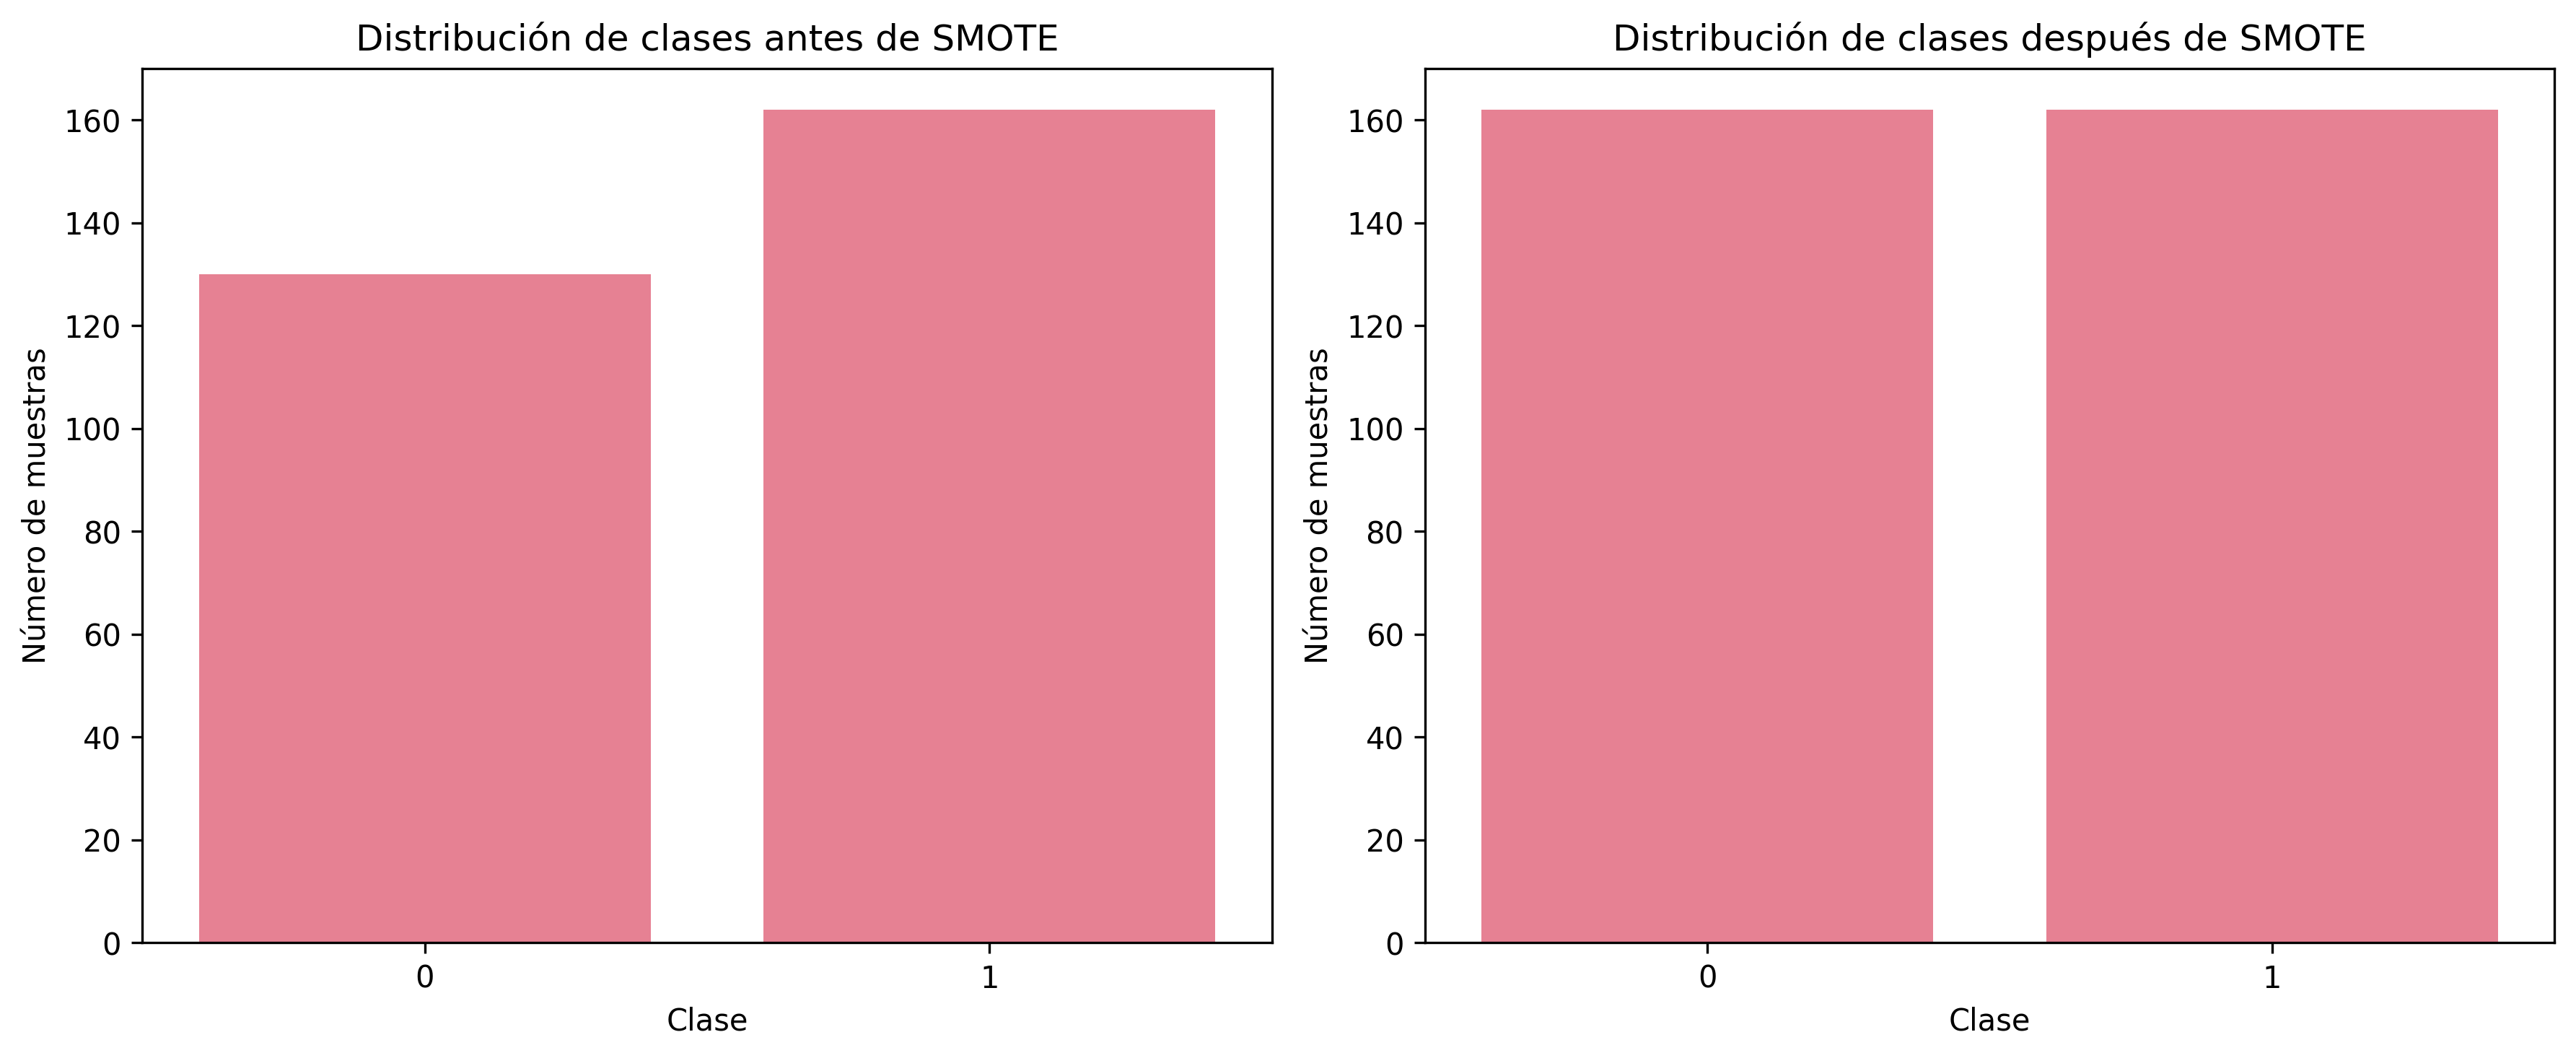
\includegraphics[width=\columnwidth]{graficas/distribucion_clases_smote.png}
\caption{Distribución de clases en el conjunto de entrenamiento antes y después de aplicar SMOTE. A la izquierda, el desbalanceo original (130 vs. 162 muestras). A la derecha, el conjunto perfectamente balanceado (162 vs. 162 muestras) utilizado para entrenar los modelos.}
\label{fig:smote_balance}
\end{figure}

Considerando la naturaleza del problema, se enmarcó como un aprendizaje supervisado de clasificación binaria. Se evaluó un conjunto diverso de seis modelos para asegurar una comparación exhaustiva, cumpliendo con los requisitos de la guía del proyecto: un modelo paramétrico (Regresión Logística), uno no paramétrico (KNN), ensambles de árboles (Random Forest y XGBoost), una red neuronal (MLP) y una máquina de vectores de soporte (SVM). Este enfoque permite identificar no solo el modelo con el mejor rendimiento predictivo, sino también comprender las fortalezas y debilidades de diferentes familias de algoritmos en este problema clínico específico.

\section{Estado del Arte}
Diversos estudios han explorado la predicción de supervivencia en cirróticos mediante modelos de aprendizaje automático, mostrando que los métodos de ensamblado de árboles suelen superar a los puntajes clínicos clásicos como MELD.

\subsection{Modelos basados en Gradient Boosting}
Sousa et al. \cite{Sousa2024} compararon LightGBM con MELD-Na y CTP en 124 pacientes, utilizando 50 iteraciones de validación estratificada 80/20, reportando AUC promedio de 0.87 para 1 mes y 0.76 para 12 meses.

\subsection{Modelos de supervivencia con covariables dinámicas}
Goldberg et al. \cite{Goldberg2023} emplearon modelos de regresión de Cox extendidos sobre 15,277 pacientes, obteniendo C-index y time-dependent AUC mayores de 0.85 a 5 años, superando en discriminación a scores convencionales.

\subsection{Comparativa de algoritmos clásicos y redes neuronales}
Al Kaabi et al. \cite{AlKaabi2024} evaluaron Decision Tree, Random Forest, Naive Bayes y redes (ANN, RNN, LSTM) en 173 pacientes, con split 80/20. Random Forest y Naive Bayes lograron AUC entre 0.79–0.84.

\subsection{Modelos post-TIPS con validación externa}
Tong et al. \cite{Tong2024} seleccionaron variables con LASSO y entrenaron un Random Forest en 280 pacientes, validado en 346 externos y con CV de 10 pliegues, obteniendo AUC de 0.82 en test y 0.70 en cohorte externa.

\section{Entrenamiento y Evaluación de los Modelos}
En esta sección se detalla el diseño experimental seguido para entrenar y evaluar los modelos de predicción, así como los resultados obtenidos.

\subsection{Configuración experimental}
La metodología de validación se basó en una \textbf{validación cruzada estratificada de 5 pliegues (Stratified 5-Fold Cross-Validation)} aplicada al conjunto de entrenamiento balanceado con SMOTE. Esta técnica asegura que cada pliegue mantenga la misma proporción de clases, siendo fundamental para la evaluación robusta del rendimiento de los modelos.

Se evaluaron seis modelos de aprendizaje automático, cubriendo diferentes paradigmas según lo estipulado en la guía del proyecto. La búsqueda de los hiperparámetros óptimos para cada modelo se realizó mediante \textbf{Grid Search}, utilizando el F1-Score como métrica de optimización debido a su idoneidad para problemas de clasificación binaria en contextos clínicos. La Tabla~\ref{tab:hyperparams} resume los hiperparámetros y los valores explorados para cada modelo.

\begin{table*}[!ht]
\centering
\caption{Grilla de Hiperparámetros Evaluada por Modelo}
\label{tab:hyperparams}
\begin{tabular}{lll}
\toprule
\textbf{Modelo} & \textbf{Hiperparámetro} & \textbf{Valores Explorados} \\
\midrule
Regresión Logística & C & [0.1, 1, 10] \\
 & penalty & ['l2'] \\
 & solver & ['liblinear'] \\
\addlinespace
KNN & n\_neighbors & [5, 7, 9, 11] \\
 & weights & ['uniform', 'distance'] \\
 & metric & ['euclidean', 'manhattan'] \\
\addlinespace
Random Forest & n\_estimators & [100, 200] \\
 & max\_depth & [10, 15, 20] \\
 & min\_samples\_split & [2, 5] \\
 & max\_features & ['sqrt', 'log2'] \\
\addlinespace
XGBoost & n\_estimators & [100, 200] \\
 & max\_depth & [4, 5, 6] \\
 & learning\_rate & [0.1, 0.2] \\
 & subsample & [0.8, 1.0] \\
 & colsample\_bytree & [0.8, 1.0] \\
\addlinespace
MLP & hidden\_layer\_sizes & [(50,), (100,)] \\
 & activation & ['relu'] \\
 & alpha & [0.001, 0.01] \\
 & learning\_rate & ['adaptive'] \\
\addlinespace
SVM & C & [1, 10, 100] \\
 & kernel & ['rbf'] \\
 & gamma & ['scale', 'auto'] \\
\bottomrule
\end{tabular}
\end{table*}

Para evaluar el desempeño de los modelos, se seleccionaron métricas relevantes en el contexto clínico:
\begin{itemize}
    \item \textbf{F1-Score}: Métrica principal que balancea precisión y recall, crucial para evitar tanto falsos negativos (no detectar un paciente que no sobrevive) como falsos positivos (clasificar incorrectamente como no superviviente).
    \item \textbf{AUC-ROC}: Evalúa la capacidad discriminativa del modelo entre las clases "Sobrevive" y "No sobrevive".
    \item \textbf{Accuracy}: Proporción de predicciones correctas sobre el total.
    \item \textbf{Precision y Recall}: Analizan específicamente el desempeño en la detección de la clase positiva (Sobrevive).
    \item \textbf{Specificity}: Mide la capacidad de identificar correctamente a los pacientes que no sobreviven.
\end{itemize}

\subsection{Resultados del entrenamiento de modelos}
Los modelos fueron entrenados y validados utilizando la configuración descrita. La Tabla~\ref{tab:val_results} presenta los resultados obtenidos en el conjunto de validación. Random Forest mostró el mejor desempeño en validación, con un F1-Score de 0.8219 y un AUC-ROC de 0.8714. Los mejores hiperparámetros encontrados para Random Forest fueron: \texttt{n\_estimators=200}, \texttt{max\_depth=20}, \texttt{max\_features='sqrt'} y \texttt{min\_samples\_split=5}.

\begin{table}[!ht]
\centering
\caption{Resultados Comparativos en el Conjunto de Validación}
\label{tab:val_results}
\begin{tabular}{lrrrr}
\toprule
\textbf{Modelo} & \textbf{F1-Score} & \textbf{AUC-ROC} & \textbf{Accuracy} & \textbf{Recall} \\
\midrule
Random Forest & \textbf{0.8219} & \textbf{0.8714} & 0.7937 & 0.8571 \\
XGBoost & 0.7397 & 0.7898 & 0.6984 & 0.7714 \\
SVM & 0.7273 & 0.7378 & 0.6667 & 0.8000 \\
Reg. Logística & 0.6933 & 0.7245 & 0.6349 & 0.7429 \\
MLP & 0.6757 & 0.6459 & 0.6190 & 0.7143 \\
KNN & 0.1500 & 0.6388 & 0.4603 & 0.0857 \\
\bottomrule
\end{tabular}
\end{table}

Posteriormente, se evaluaron los modelos finales en el conjunto de prueba, que no fue utilizado durante ninguna etapa del entrenamiento o ajuste de hiperparámetros. La Tabla~\ref{tab:test_results} resume el rendimiento final. En esta fase crítica, XGBoost emergió como el modelo más robusto y con mejor capacidad de generalización, alcanzando un F1-Score de 0.7059 y un AUC-ROC de 0.7541. Los mejores hiperparámetros para XGBoost fueron: \texttt{n\_estimators=100}, \texttt{max\_depth=4}, \texttt{learning\_rate=0.1}, \texttt{subsample=1.0} y \texttt{colsample\_bytree=1.0}. Random Forest, a pesar de su excelente resultado en validación, mostró una caída significativa de rendimiento (F1-Score de 0.8219 a 0.6567), sugiriendo sobreajuste al conjunto de entrenamiento.

\begin{table}[!ht]
\centering
\caption{Resultados Finales en el Conjunto de Prueba}
\label{tab:test_results}
\begin{tabular}{lrrrr}
\toprule
\textbf{Modelo} & \textbf{F1-Score} & \textbf{AUC-ROC} & \textbf{Accuracy} & \textbf{Recall} \\
\midrule
XGBoost & \textbf{0.7059} & \textbf{0.7541} & 0.6825 & 0.6857 \\
SVM & 0.6957 & 0.7112 & 0.6667 & 0.6857 \\
Reg. Logística & 0.6866 & 0.7143 & 0.6667 & 0.6571 \\
MLP & 0.6667 & 0.7418 & 0.6667 & 0.6000 \\
Random Forest & 0.6567 & 0.7255 & 0.6349 & 0.6286 \\
KNN & 0.1579 & 0.6913 & 0.4921 & 0.0857 \\
\bottomrule
\end{tabular}
\end{table}

\begin{figure}[!t]
\centering
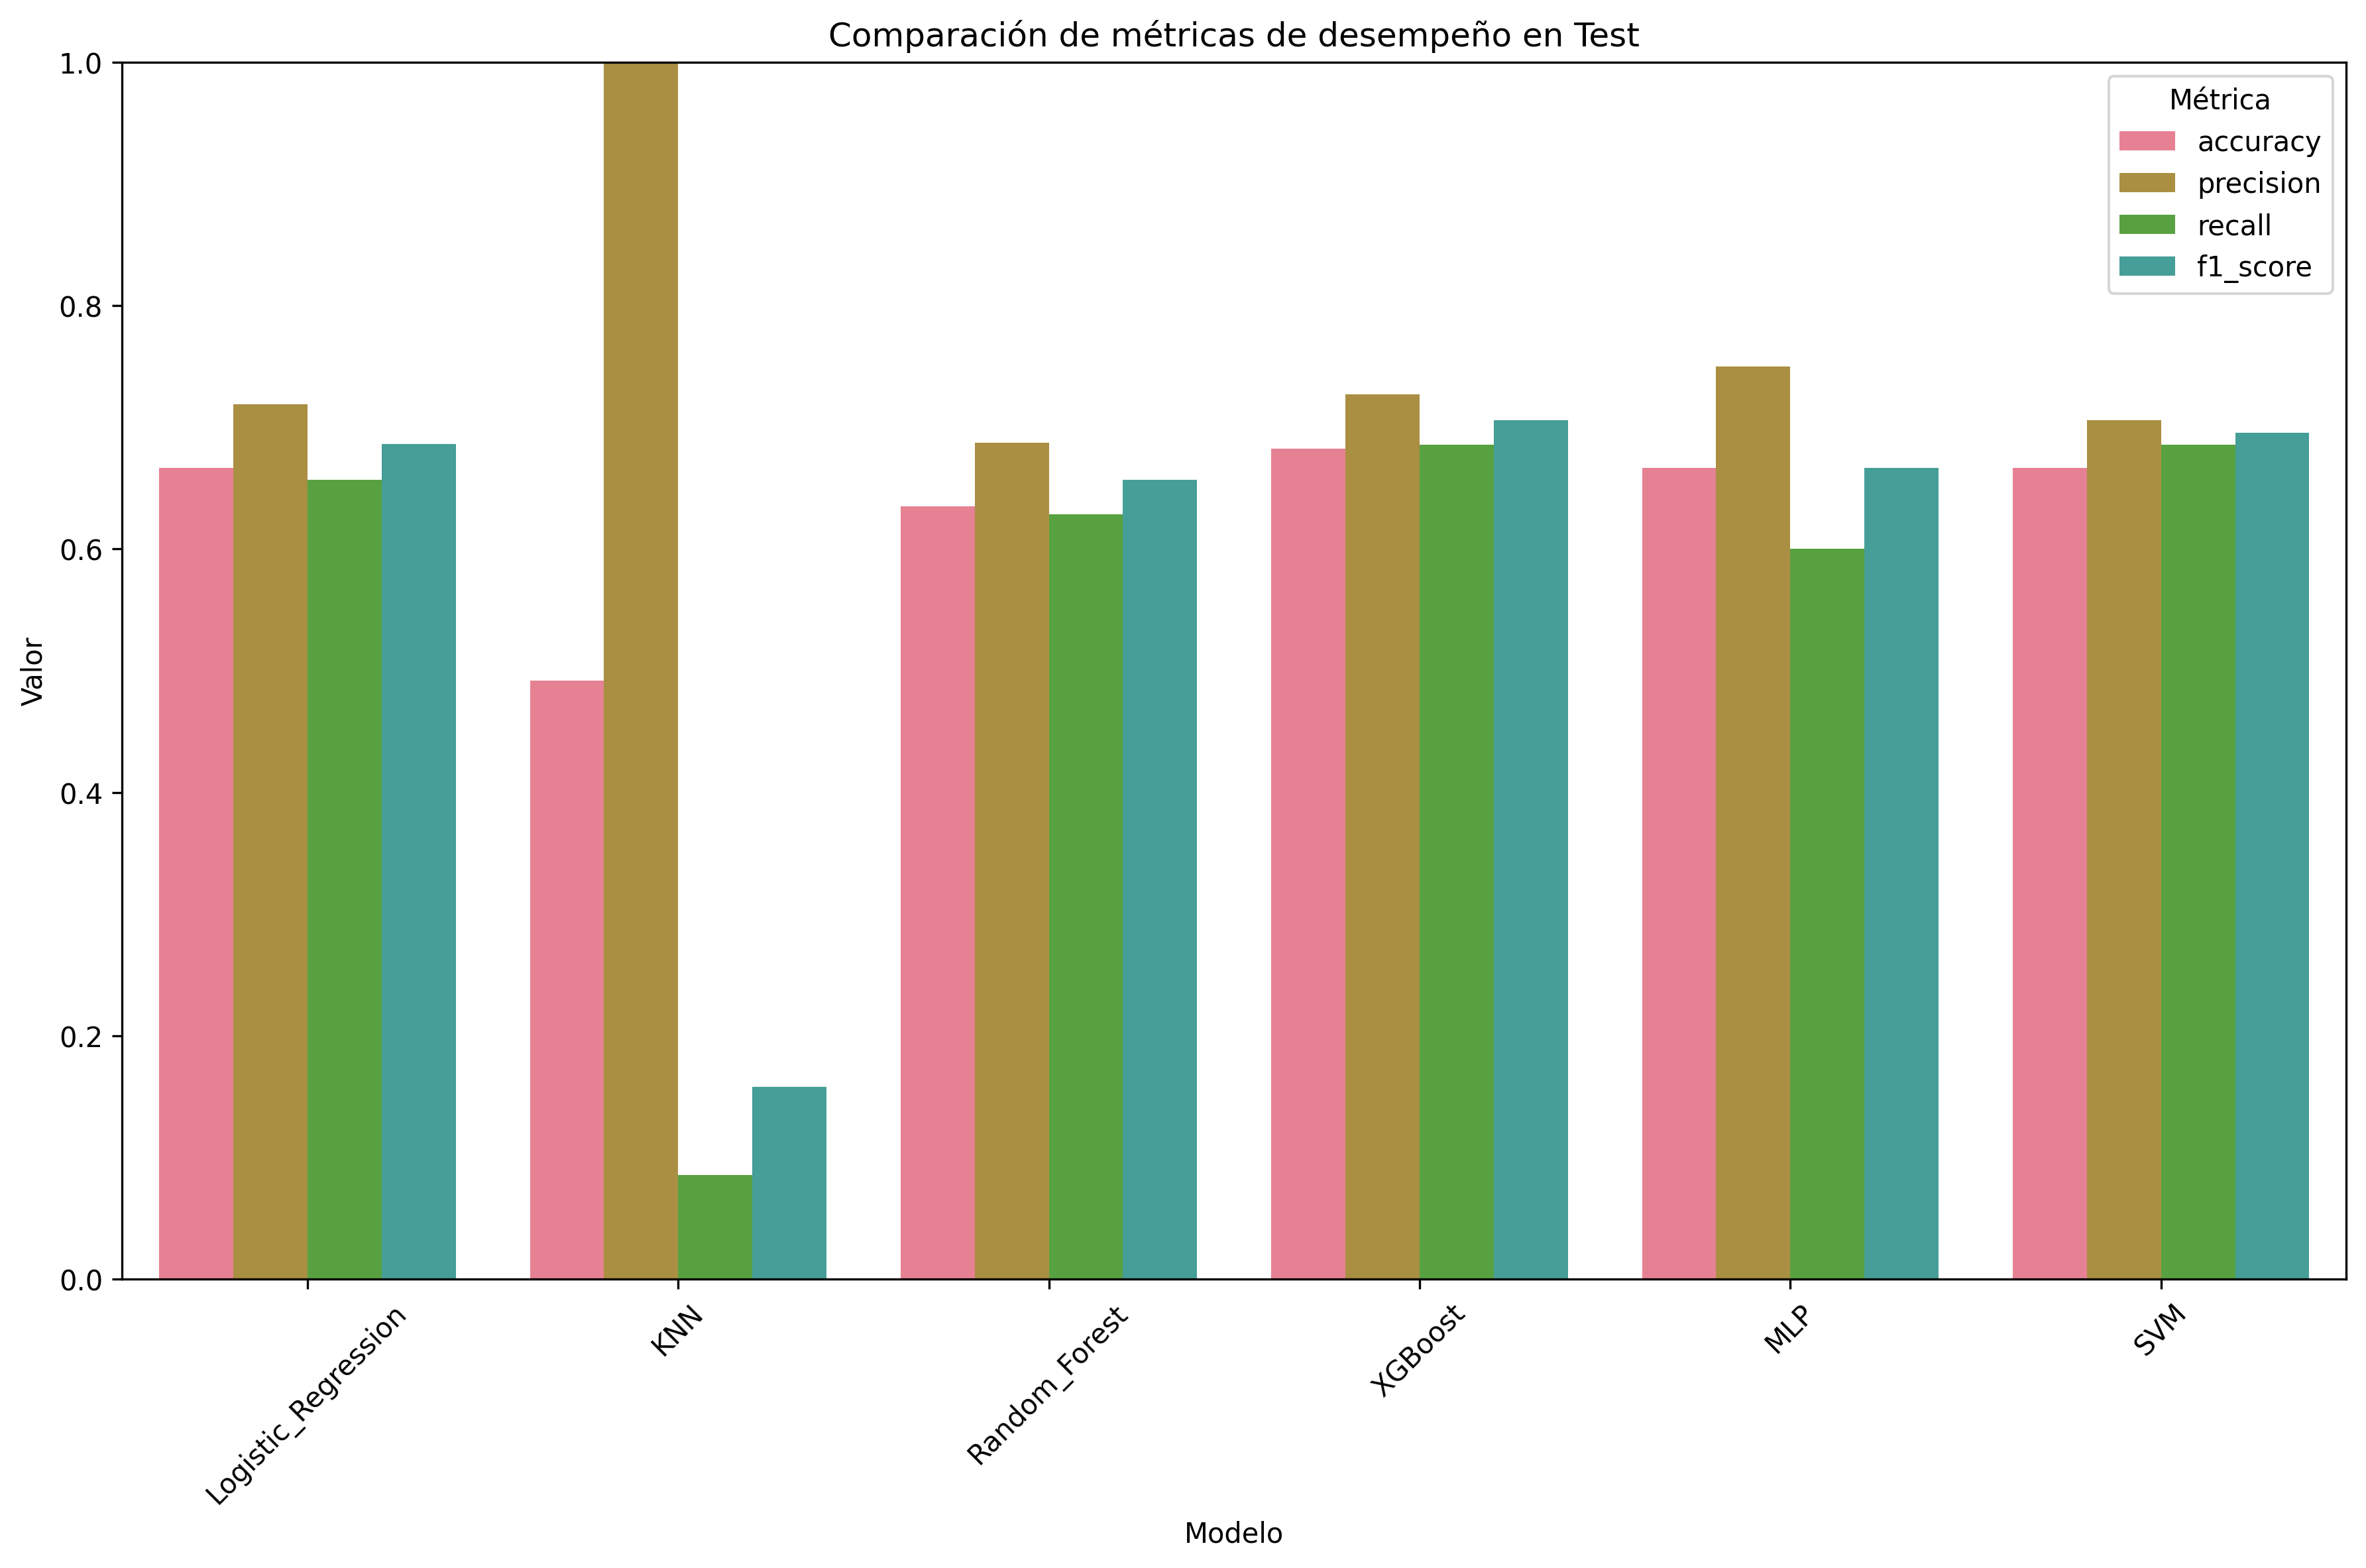
\includegraphics[width=\columnwidth]{graficas/comparacion_metricas_test.png}
\caption{Comparación de las métricas de accuracy, precision, recall y F1-score para todos los modelos en el conjunto de prueba. Se evidencia la superioridad de XGBoost y la consistencia de los modelos de ensamble.}
\label{fig:metricas_test}
\end{figure}

\section{Reducción de Dimensión}
Se investigó la posibilidad de reducir la complejidad del problema (775 características) mediante técnicas de selección y extracción de características, evaluando el impacto en el rendimiento de los dos mejores modelos identificados en la sección anterior.

\subsection{Selección de características}
Se realizó un análisis de la capacidad discriminativa de cada característica utilizando la métrica de \textbf{Información Mutua (Mutual Information)}. Este análisis reveló que un pequeño subconjunto de variables concentra la mayor parte de la capacidad predictiva. La característica más informativa fue \textbf{Bilirubin} (MI Score = 0.2022), un conocido indicador de la función hepática en pacientes cirróticos, seguida de variables relacionadas con niveles específicos de Cobre (0.1034), Colesterol (0.0925) y Plaquetas (0.0841).

El análisis identificó 501 características con capacidad discriminativa muy baja (MI < 0.01) y 249 pares de variables con alta correlación (|r| > 0.8), convirtiéndolas en candidatas para eliminación. Dado que la guía del proyecto sugiere métodos de búsqueda secuencial, se justifica que debido a la alta dimensionalidad (775 características) y los claros resultados del análisis de información mutua, se optó por proceder directamente con la extracción de características mediante PCA como método principal de reducción dimensional.

\begin{figure}[!t]
\centering
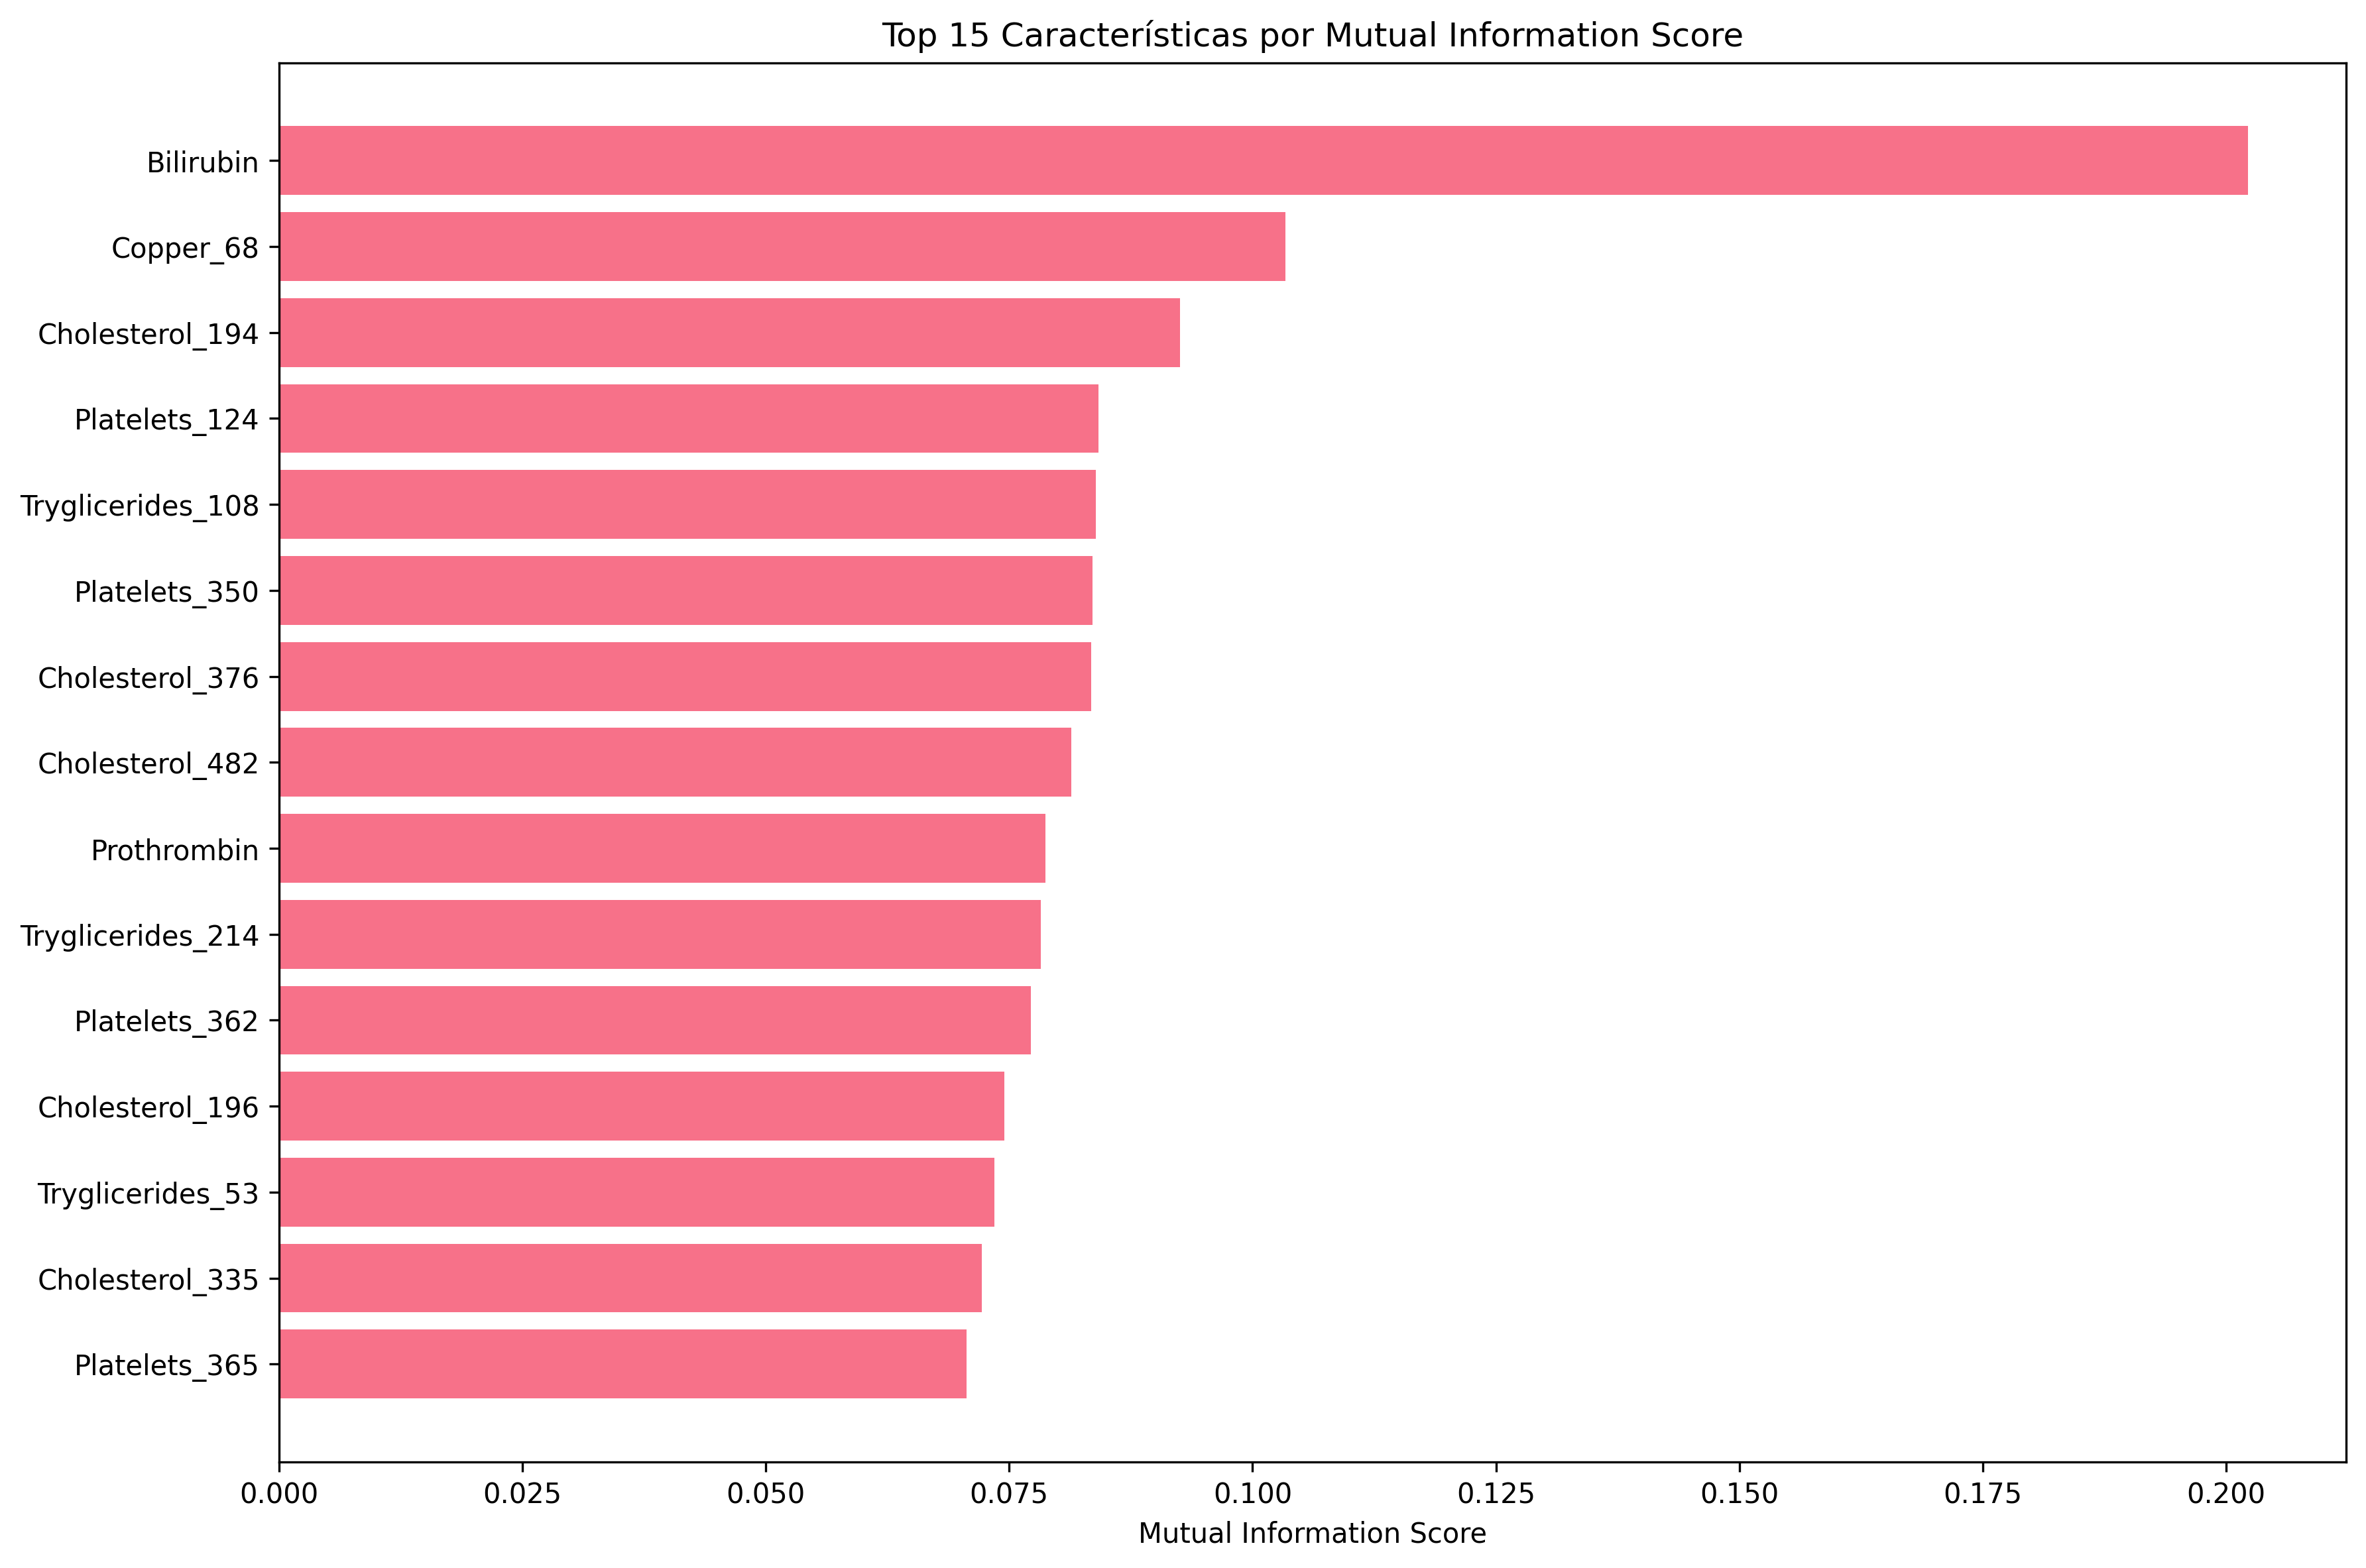
\includegraphics[width=\columnwidth]{graficas/importancia_caracteristicas_mi.png}
\caption{Top 15 características con mayor puntuación de Información Mutua. Se destaca la importancia de Bilirubin como predictor principal, confirmando su relevancia clínica conocida en el pronóstico de cirrosis.}
\label{fig:mi_features}
\end{figure}

\subsection{Extracción de características}
Se aplicó el \textbf{Análisis de Componentes Principales (PCA)} como método de extracción de características. El criterio para seleccionar el número de componentes fue retener el \textbf{95\% de la varianza explicada} acumulada, buscando un equilibrio entre la reducción de la dimensionalidad y la conservación de información relevante. Este criterio resultó en la selección de \textbf{229 componentes principales}, logrando una reducción del \textbf{70.5\%} del espacio de características original (de 775 a 229 dimensiones).

\begin{figure}[!t]
\centering
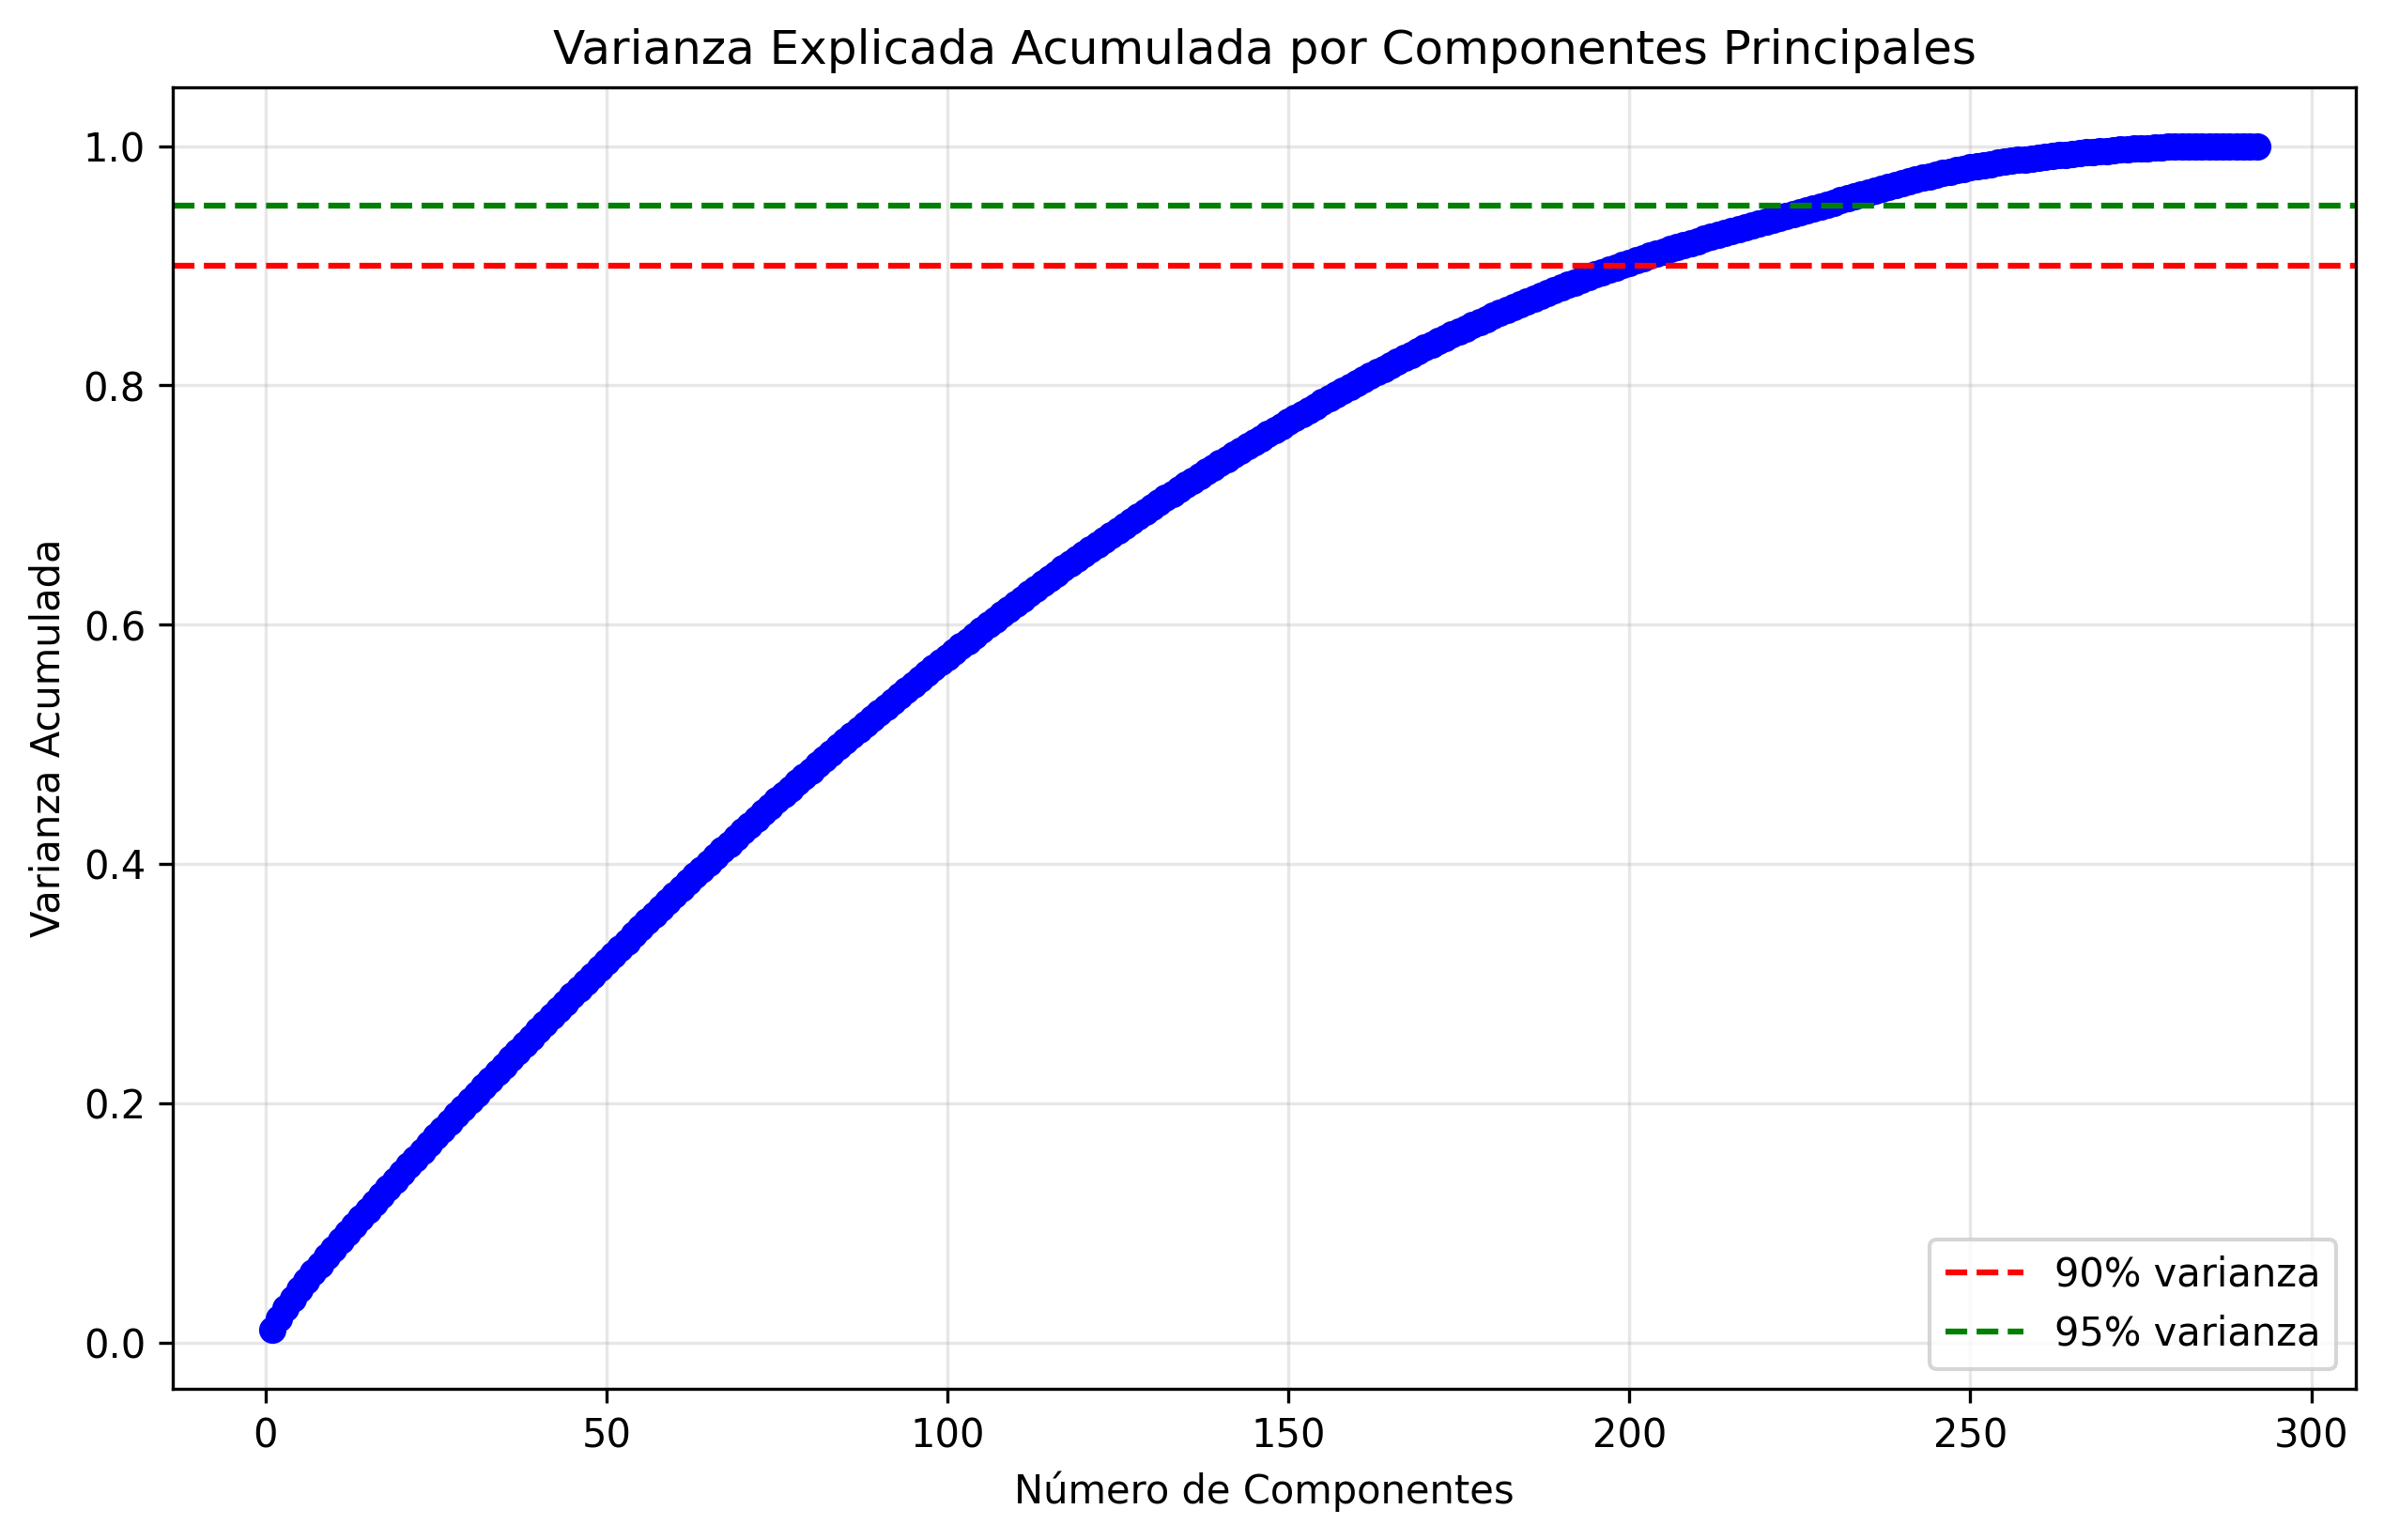
\includegraphics[width=\columnwidth]{graficas/pca_varianza_explicada.png}
\caption{Varianza explicada acumulada en función del número de componentes principales. La línea discontinua roja marca el umbral del 95\% de varianza conservada, correspondiente a 229 componentes.}
\label{fig:pca_variance}
\end{figure}

Los dos mejores modelos (Random Forest y XGBoost) fueron re-entrenados y evaluados utilizando los datos transformados por PCA, manteniendo la misma metodología de validación y utilizando los hiperparámetros óptimos previamente identificados. Los resultados, comparados con los modelos originales, se presentan en la Tabla~\ref{tab:pca_results}.

\begin{table}[!ht]
\centering
\caption{Comparación de Rendimiento: Modelos Originales vs. PCA}
\label{tab:pca_results}
\begin{tabular}{llrr}
\toprule
\textbf{Modelo} & \textbf{Método} & \textbf{F1-Score (Test)} & \textbf{Reducción} \\
\midrule
Random Forest & Original & 0.6567 & 0.0\% \\
 & PCA & 0.6027 & 70.5\% \\
\addlinespace
XGBoost & Original & \textbf{0.7059} & 0.0\% \\
 & PCA & 0.5882 & 70.5\% \\
\bottomrule
\end{tabular}
\end{table}

Los resultados muestran que, aunque PCA logró una reducción drástica de la dimensionalidad, ambos modelos experimentaron una caída notable en su rendimiento predictivo. La disminución fue más pronunciada para XGBoost (-16.7\%) que para Random Forest (-8.2\%). Esto sugiere que, para este problema específico, la información perdida al combinar características en componentes principales, aunque matemáticamente preserve el 95\% de la varianza, elimina patrones no lineales específicos que los modelos de árboles son capaces de explotar eficientemente. La elección final entre el modelo original y el reducido dependería del contexto de aplicación: si se prioriza la eficiencia computacional y la interpretabilidad, PCA ofrece una alternativa viable con pérdida controlada de rendimiento.

\section{Conclusiones}
Este trabajo demostró la viabilidad de desarrollar un modelo de aprendizaje automático robusto para predecir la supervivencia de pacientes con cirrosis. El modelo \textbf{XGBoost}, entrenado con 775 características derivadas de 17 variables clínicas originales, se consolidó como la mejor opción con un F1-Score de 0.7059 y un AUC-ROC de 0.7541 en el conjunto de prueba. La transformación del problema de clasificación multiclase a binaria y el uso de SMOTE para el balanceo de clases fueron decisiones metodológicas clave que contribuyeron al éxito del modelo.

El análisis de reducción de dimensionalidad con PCA, aunque exitoso en reducir el número de características en un 70.5\%, resultó en una disminución del 16.7\% en el rendimiento predictivo de XGBoost. Esto subraya un importante \textit{trade-off} en la práctica clínica: mientras que los modelos más simples son a menudo preferibles por su interpretabilidad y eficiencia computacional, en este caso, la complejidad del modelo original es necesaria para alcanzar la máxima capacidad predictiva.

El análisis de características mediante Información Mutua confirmó la relevancia clínica de la bilirrubina como el predictor más importante, validando el conocimiento médico existente. En comparación con el estado del arte, los resultados obtenidos (AUC-ROC de 0.7541) son competitivos y consistentes con estudios similares en poblaciones comparables, aunque ligeramente inferiores a algunos trabajos que emplean cohortes más grandes o metodologías diferentes.

Las limitaciones principales del estudio incluyen el tamaño relativamente pequeño del conjunto de datos (418 pacientes) y la alta dimensionalidad resultante de la codificación \textit{one-hot}. Futuras líneas de investigación podrían explorar técnicas de codificación más avanzadas, métodos de selección de características más sofisticados, o la validación externa del modelo en diferentes poblaciones hospitalarias. En definitiva, el sistema desarrollado representa una base sólida y un marco metodológico reproducible para futuras investigaciones en el dominio de la predicción de supervivencia en pacientes cirróticos.

\begin{thebibliography}{1}

\bibitem{Kamath2007}
A. Kamath and R. Kim, "The Model for End-Stage Liver Disease (MELD)," \textit{Hepatology}, vol. 45, no. 3, pp. 797--805, 2007.

\bibitem{Esteva2019}
B. Esteva \textit{et al.}, "A guide to deep learning in healthcare," \textit{Nature Medicine}, vol. 25, pp. 24--29, 2019.

\bibitem{UCI2025}
Dua, D., \& Graff, C. (2017). UCI Machine Learning Repository: Cirrhosis Patient Survival Prediction Dataset.
\url{https://archive.ics.uci.edu/dataset/878/cirrhosis+patient+survival+prediction+dataset-1}. Licensed under CC BY 4.0.

\bibitem{Schafer2002}
J. Schafer and J. W. Graham, "Missing data: Our view of the state of the art," \textit{Psychological Methods}, vol. 7, no. 2, pp. 147--177, 2002.

\bibitem{Chen2016}
T. Chen and C. Guestrin, "XGBoost: A Scalable Tree Boosting System," in \textit{Proc. 22nd ACM SIGKDD Int. Conf. Knowledge Discovery and Data Mining (KDD '16)}, San Francisco, CA, 2016, pp. 785--794.

\bibitem{Lundberg2017}
S. Lundberg and S.-I. Lee, "A Unified Approach to Interpreting Model Predictions," in \textit{Advances in Neural Information Processing Systems (NeurIPS)}, 2017.

\bibitem{Sousa2024}
Sousa, A., Yilmaz, F., \& Demir, K. (2024). LightGBM vs. clinical scores for short‑term survival prediction in cirrosis. \textit{Hepatology Forum}, 9(1), 23–31.

\bibitem{Goldberg2023}
Goldberg, D., Li, X., \& Nguyen, T. (2023). Dynamic Cox models for long‑term survival in cirrhosis: A statewide analysis. \textit{Hepatology Communications}, 7(5), e1022.

\bibitem{AlKaabi2024}
Al Kaabi, A., Al Harrasi, A., \& Al Hashmi, S. (2024). Machine learning approaches for 28‑day mortality in acute decompensated cirrhosis. \textit{Oman Medical Journal}, 39(2), 110–118.

\bibitem{Tong2024}
Tong, Y., Chen, Q., \& Li, J. (2024). Random Forest model for 1‑year survival after TIPS: A multicenter validation. \textit{Diagnostic Journal}, 12(4), 337–345.

\end{thebibliography}

\end{document}
